\subsection{Основные подходы к распараллеливанию}
\label{subsec:parallelization-approaches}

На практике сложилось достаточное большое количество шаблонов параллельного программирования.
Однако все эти шаблоны в своей основе используют три базовых подхода к распараллеливанию:

\begin{itemize}
    \item\textbf{Распараллеливание по данным:} Программист находит в программе массив данных, элементы которого программа последовательно обрабатывает в некоторой функции func.
    Затем программист пытается разбить этот массив данных на блоки, которые могут быть обработаны в func независимо друг от друга.
    Затем программист запускает сразу несколько потоков, каждый из которых выполняет func, но при этом обрабатывает в этой функции отличные от других потоков блоки данных.
    \item\textbf{Распараллеливание по инструкциям:} Программист находит в программе последовательно вызываемые функции, процесс работы которых не влияет друг на друга (такие функции не изменяют общие глобальные переменные, а результаты одной не используются в работе другой).
    Затем эти функции программист запускает в параллельных потоках.
    \item\textbf{Распараллеливание по информационным потокам:} Программа представляет собой набор выполняемых функций, причем несколько функций могут ожидать результата выполнения предыдущих.
    В таком случае каждое ядро выполняет ту функцию, данные для которой уже готовы.
    Рассмотрим этот метод на примере абстрактного двухъядерного процессора как наиболее сложный для понимания.
    Структурный алгоритм, изображенный на рисунке~\ref{fig:2-core-algorithm}, состоит из 9 функций, некоторые из которых используют результат предыдущей функции в своей работе.
    Будем считать, что функция 3 использует результат работы функции 1, а функция 7 - результат функций 4 и 6 и т.д., а также функция 5 выполняется по времени примерно столько же, сколько функции 7, 8 и 9, вместе взятые.
    Тогда на двухъядерной машине этот способ распараллеливания будет оптимальным решением.
\end{itemize}

\begin{figure}[H]
    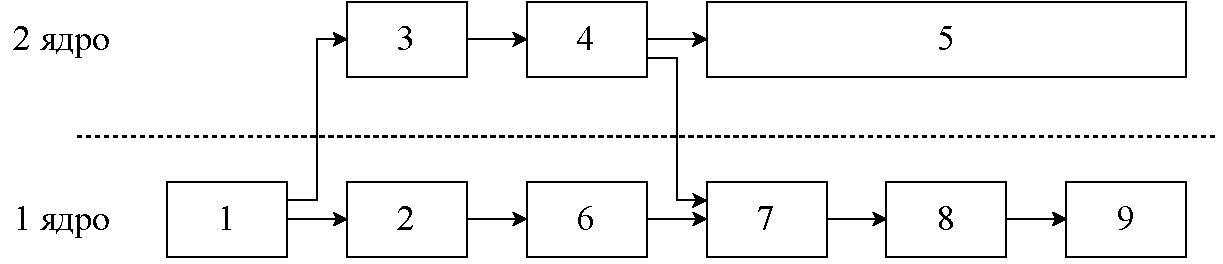
\includegraphics[width=\linewidth]{2-core_algorithm}
    \caption{Пример работы структурного алгоритма на двухъядерном процессоре}
    \label{fig:2-core-algorithm}
\end{figure}

% На практике сложилось достаточное большое количество шаблонов параллельного программирования. Однако все эти шаблоны в своей основе используют три базовых подхода к распараллеливанию: по данным, по инструкциям и по информационным потокам.

% \subsubsection*{Распараллеливание по данным}
% Программист находит в программе массив данных, элементы которого программа последовательно обрабатывает в некоторой функции func. Затем программист пытается разбить этот массив данных на блоки, которые могут быть обработаны в func независимо друг от друга. Затем программист запускает сразу несколько потоков, каждый из которых выполняет func, но при этом обрабатывает в этой функции отличные от других потоков блоки данных.

% \subsubsection*{Распараллеливание по инструкциям}
% Программист находит в программе последовательно вызываемые функции, процесс работы которых не влияет друг на друга (такие функции не изменяют общие глобальные переменные, а результаты одной не используются в работе другой). Затем эти функции программист запускает в параллельных потоках.

% \subsubsection*{Распараллеливание по информационным потокам}
% Программа представляет собой набор выполняемых функций, причем несколько функций могут ожидать результата выполнения предыдущих. В таком случае каждое ядро выполняет ту функцию, данные для которой уже готовы. Рассмотрим этот метод на примере абстрактного двухъядерного процессора, как наиболее сложный для понимания. Структурный алгоритм, изображенный на рисунке~\ref{structAlgorithm:image} состоит из 9 функций, некоторые из которых используют результат предыдущей функции в своей работе. Будем считать, что функция 3 использует результат работы функции 1, а функция 7 -- результат функций 4 и 6 и т.д., а также функция 5 выполняется по времени примерно столько же сколько функции 7, 8 и 9, вместе взятые. Тогда, на двухъядерной машине этот способ распараллеливания будет оптимальным решением.

% \begin{figure}[H]
%     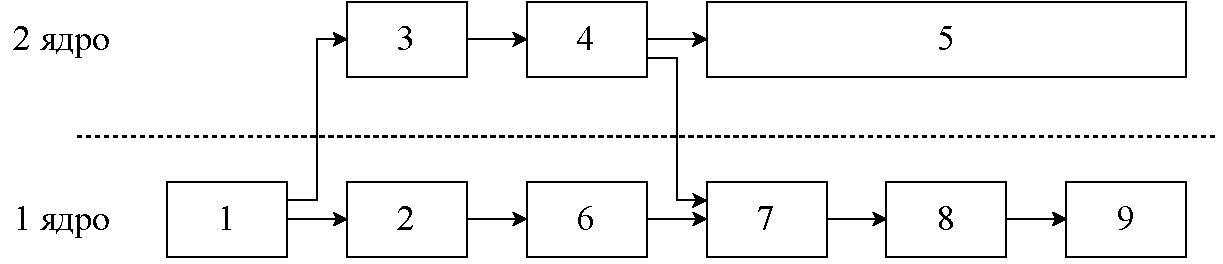
\includegraphics[width=\linewidth]{2-core_algorithm}
%     \caption{Пример работы структурного алгоритма на двухъядерном процессоре}
%     \label{structAlgorithm:image}
% \end{figure}

Три описанных метода легче понять на аналогии из обыденной жизни.
Пусть два студента получили в стройотряде задание подмести улицу и покрасить забор.
Если студенты решат использовать распараллеливание по данным, он будут сначала вместе подметать улицу, а затем вместе же красить забор.
Если они решат использовать распараллеливание по инструкциям, то один студент полностью подметёт улицу, а другой покрасит в это время весь забор.
Распараллелить по информационным потокам эту ситуацию не получится, так как эти два действия никак не зависят друг от друга.
Если предположить, что им обоим нужны инструменты для работы, то один из них должен сначала сходить за ними, а потом они оба начнут делать свою работу.

В большем числе случаев решение об использовании метода является очевидным в силу внутренних особенностей распараллеливаемой программы.
Выбор метода определяется тем, какой из них более равномерно загружает потоки.
В идеале все потоки должны приблизительно одновременно заканчивать выделенную им работу, чтобы оптимально загрузить ядра (процессоры) и чтобы закончившие работу потоки не простаивали в ожидании завершения работы соседними потоками.
